\documentclass{article}
% \usepackage{hyperref}

\usepackage{titlesec}
\usepackage{titling}
\usepackage{multicol}
% \usepackage{hyperref}
\usepackage[margin=0.2in]{geometry}

\usepackage{MnSymbol}
\usepackage{amsmath} 
\usepackage{graphicx} 
\usepackage{eso-pic}
\usepackage[hidelinks]{hyperref}

\hypersetup{
    colorlinks=true,
    linkcolor=blue,
    filecolor=magenta,      
    urlcolor=[rgb]{0,0,1},
    pdftitle={Kaustav-Resume},
    % pdfpagemode=FullScreen,
    }


\usepackage{ifthen}
\newboolean{showProjectlinks}
\setboolean{showProjectlinks}{true}


\titleformat{\section}
{\large\uppercase}
{}
{0em}
{}[\titlerule]

\titleformat{\subsection}[runin]
{\bfseries}
{}
{1em}
{}[]

%%%%%%%%%%%%%%%%   Make Title for Heading Style 1  %%%%%%%%%%%%%%%%

% \renewcommand{\maketitle}{
%     \begin{flushleft}        
%         {\huge\rmfamily
%         \theauthor}\newline
%         \vspace{0.1em}
%         \textmd{teetangh@gmail.com -- github.com/teetangh}\newline
%         \textmd{Contact No. -- +91-8800441954}\newline
%         \textmd{Manipal Institute of Technology}\newline
%         \textmd{B.Tech in \textbf{Computer Science \& Engineering}}
%         \textmd{2018 - 2022}\newline
%         \textmd{Minor in \textbf{Computational Intelligence}}\newline
%         \textmd{CGPA: 8.54/10}\newline
%         \href{https://www.github.com/teetangh}{GitHub} \
%         \href{https://www.linkedin.com/in/kaustav-ghosh-1538651bb/}{LinkedIn}
%     \end{flushleft}
% }


\titlespacing*{\subsection}
{0em}
{0em}
{0em}


%%%%%%%%%%%%%%%%%%%%%%%%%%%%%%%%%%%%%%   DOCUMENT  %%%%%%%%%%%%%%%%%%%%%%%%%%%%%%%%%%%%%%


%%%%%%%%%%%%%%%%   Heading Style 1  %%%%%%%%%%%%%%%%

\begin{document}
\thispagestyle{empty}  % for no page numbering

% \begin{multicols}{2}
%     \title{Resume}
%     \author{Kaustav Ghosh}
%     \maketitle
%     \begin{flushright}
%         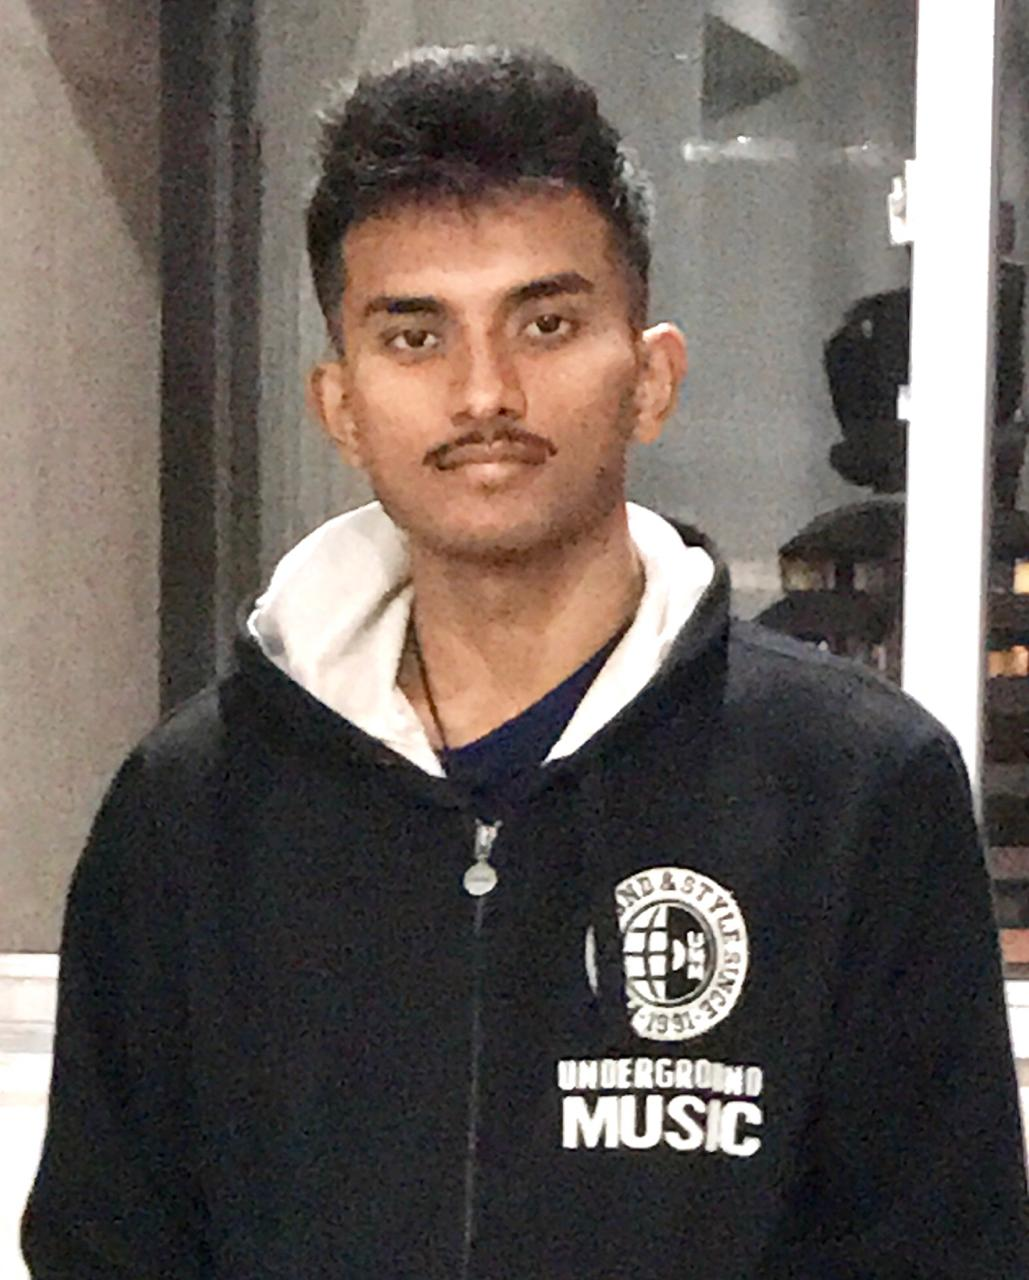
\includegraphics[height=3cm]{kaustav2.jpeg}
%     \end{flushright}
% \end{multicols}


%%%%%%%%%%%%%%%%   Heading Style 2  %%%%%%%%%%%%%%%%

\begin{center}
    \huge{Kaustav Ghosh} % TODO: LEAVE A BLANK LINE AFTER THIS

    \normalsize{
        \textmd{
            \href{https://www.github.com/teetangh}{GitHub} \(|\)
            \href{https://www.linkedin.com/in/kaustav-ghosh-1538651bb/}{LinkedIn} \(|\)
            teetangh@gmail.com \(|\)
            Gugraon,India \(|\)
            +91-8800441954
        }}
\end{center}

%%%%%%%%%%%%%%%%%%%%%%%%%%%%%%%%%%%%%%   Education  %%%%%%%%%%%%%%%%%%%%%%%%%%%%%%%%%%%%%%

\section*{Education}

\textbf{Manipal Institute of Technology} \hfill \textmd{2018-2022}
\textmd{\newline \textmd{BTech in Computer Science \& Engineering specializing in Computational Intelligence}}
% \textmd{\newline \textmd{Interests: Artificial Intelligence and Robotics}}
\ifthenelse{\boolean{showProjectlinks}}{\textbf{Lab Work:}
    \href{https://github.com/teetangh/Kaustav-CSE-LABS-and-Projects}{\text{[Repository]}}.
}{}
\hfill \textmd{CGPA: 8.57/10}
\newline
\textmd{\textbf{Courses Taken:} Database Management Systems, Operating System, Computer Networking, Software Engineering, Object-Oriented Analysis And Design(OOPs), Digital Logic Design, Distributed Systems, Computer Organization And Architecture}

%%%%%%%%%%%%%%%%%%%%%%%%%%%%%%%%%%%%%%   Work Experience  %%%%%%%%%%%%%%%%%%%%%%%%%%%%%%%%%%%%%%

\section*{Work Experience}

\begin{itemize}

    \item{\textbf{\large{Hevo Data, Bangalore - Software Development Engineer Intern}}} \hfill \textmd{Jan'22-Jun'22}
          \newline
          \textmd{- Worked in the backend integrations team where I designed and implemented an end-to-end \textbf{REST API connector} and \textbf{SDK} for the data source, Braze, a software as a service (SaaS) platform, by deciding the source objects, the polling strategies, building the SDK authentication, models, client, and the connector offset, tasks, and services for polling each source object.}
          \newline
          \textmd{- Worked on debugging several issues on already existing connectors tracked by \textbf{Sentry} and \textbf{Coralogix}, wrote suitable documentation and developed unit tests for Outbrain using \textbf{JUnit5} and \textbf{Mockito} and which were subject to code review.}
          \newline 
          \textmd{- Worked on resolving Google Big-Query and Marketo On-call issues supported with Senior developers}

    \item{\textbf{\large{Samsung R\&D, Bangalore - Software Development Engineer Intern}}} \hfill \textmd{Jun'21-Jul'21}
          \newline
          \textmd{- Designed and implemented \textbf{MQTT bridge functionality} in Moquette, an open-source lightweight Java MQTT broker}
          \newline
          \textmd{- Implemented a \textbf{socket programming system} for the transfer of messages between the MQTT message broker and the bridge client and also a \textbf{lexical analyzer} to parse the user-specified configuration of the bridge properties and the bridge client}
          % \item{\textbf{\large{Microsoft Student Partners - Machine Learning Intern}}} \hfill \textmd{Apr'20-Jun'20}
          %       \newline
          %       \textmd{- Guided a team of 10 individuals to collaborate and accomplish a Regression task of price prediction of used cars in a machine learning pipeline through Exploratory Data Analysis, Feature Engineering and Model Building.}
          %       \ifthenelse{\boolean{showProjectlinks}}{
          %           \textbf{Projects:}\href{https://nbviewer.jupyter.org/github/teetangh/Microsoft-Student-Partners-Machine-Learning-Internship/blob/main/MINOR\%20PROJECT/Microsoft_Minor_Project_v2.ipynb}{\text{[Minor]}}.
          %           \href{https://nbviewer.jupyter.org/github/Microsoft-ML-Internship-Team/Major-Project-Submissions/tree/master/KAUSTAV/}{\text{[Major]}}.
          %       }{}

          % \item{\textbf{\large{TakenMind Technologies - Data Analytics Intern}}}\hfill \textmd{May'20}
          %       \newline
          %       \textmd{- Worked on analyzing Industrial Data, predicting and presenting trends, using techniques such as Exploratory Data Analysis and Data visualization using Matplotlib and Seaborn. Implemented several bar plots, heatmaps, etc on several datasets. Implemented Machine Learning Algorithms (such as Random Forests). Obtained 87\% test accuracy.}
          %       \ifthenelse{\boolean{showProjectlinks}}{\textbf{Source Code:}
          %           \href{https://nbviewer.jupyter.org/github/Kaggle-Workspace/UN-SDG-Takenmind-Internship-IBM-Employee-Attrition/blob/main/Major\%20Assignment/Predicition.ipynb}{\text{[Notebook]}}.
          %       }{}

\end{itemize}


%%%%%%%%%%%%%%%%%%%%%%%%%%%%%%%%%%%%%%   Research Work  %%%%%%%%%%%%%%%%%%%%%%%%%%%%%%%%%%%%%%

\section*{Research Work}
\begin{itemize}
    % \item{\textbf{\large{Samsung - Intelligent Ranking for Dynamic Restoration in Wireless Networks}}} \hfill \textmd{Sep'20-Mar'21}
    \item{\textbf{\large{Samsung PRISM - Machine Learning Intern}}} \hfill \textmd{Sep'20-Mar'21}
          \newline
          \textbf{Intelligent Ranking for Dynamic Restoration of Next Generation Wireless Networks}
          \newline
          \textmd{- Implemented Machine Learning algorithms and Feature Engineering techniques to predict KPI values for eNodeB-s and consequently a ranking system to orderly restore them during a network failure.}
\end{itemize}

%%%%%%%%%%%%%%%%%%%%%%%%%%%%%%%%%%%%%%   Projects  %%%%%%%%%%%%%%%%%%%%%%%%%%%%%%%%%%%%%%

\section*{Projects}
\begin{itemize}

    \item{\textbf{\large{Noteups - A Lecture Notes sharing platform} \ifthenelse{\boolean{showProjectlinks}}{\href{https://github.com/The-Developer-Bros/noteups_web_original}{\text{[Repository]}}.}{}}}
          \newline
          \textmd{- Implemented the front-end using \textbf{ReactJS, Redux Toolkit and RTK Query} for state management, \textbf{Framer Motion} for animations and \textbf{Styled Components} for styling, \textbf{Media Queries} for responsive design, \textbf{Sass} for CSS pre-processing}
          \newline
          \textmd{- Implemented the back-end using \textbf{NodeJS} and \textbf{ExpressJS} for server-side rendering, used \textbf{MongoDB} as a non-relational(NoSQL) database and, Cloudinary for images storage and \textbf{PassportJS} for JWT and OAuth authentication.}
          \newline
          %   \textmd{- Created an encrypted PDF-viewer using PDF.js and ReactPDF for PDF rendering.}
          \textmd{- Implemented functionality to synchronize the note products between \textbf{Cloudinary} and \textbf{MongoDB}. and integrated \textbf{Stripe} for payment processing and working on integrating Razorpay.}
          \newline
          \textmd{- Deployed on the cloud with the frontend on \textbf{Netlify} and the backend on \textbf{Heroku}.}
          \ifthenelse{\boolean{showProjectlinks}}{\textbf{Deployed Links:}
              \href{https://noteups-frontend.netlify.app/}{\text{[Frontend]}}
              \textbf{}
              \href{https://noteups-backend.herokuapp.com/}{\text{[Backend]}}.
          }{}

    \item{\textbf{\large{Freelancing standalone web development projects}}}
          \newline
          \textmd{- Implemented a JSON Web Token Authentication system for a \textbf{NodeJS} backend.}
          \ifthenelse{\boolean{showProjectlinks}}{\textbf{}
              \href{https://github.com/Developement-Practice/reunion-assignment/blob/master/src/app.js}{\text{[Project]}}.
          }{}
          \newline
          \textmd{- Developed a Movie-Ticket booking website using \textbf{MongoDB, Nodejs and Express.}}
          \ifthenelse{\boolean{showProjectlinks}}{\textbf{}
              \href{https://github.com/Developement-Practice/fliptree-assignment/blob/main/server.js}
              {\text{[Project]}}.
          }{}
          \newline
          \textmd{- Developed a project management application using \textbf{Python, PostgreSQL, and psycopg2.}}
          \ifthenelse{\boolean{showProjectlinks}}{\textbf{}
              \href{https://github.com/Developement-Practice/factwise-assignment}
              {\text{[Project]}}.
          }{}
          \newline
          \textmd{- Developed a horizontal non-linear stepper form using \textbf{ReactJS}}
          \ifthenelse{\boolean{showProjectlinks}}{\textbf{}
              \href{https://github.com/Developement-Practice/altimate-assignment/blob/main/frontend/src/components/HorizontalNonLinearStepper.jsx}
              {\text{[Project]}}.
          }{}


    \item{\textbf{\large{Microsoft Student Partners - Machine Learning Bootcamp}}}
          \newline
          \textmd{- Demonstrated leadership skills by mentoring a team of 10 individuals to accomplish a Regression task of price prediction of  cars in a machine learning pipeline through Exploratory Data Analysis, Feature Engineering and Model Building.}
          \ifthenelse{\boolean{showProjectlinks}}{
              \textbf{}\href{https://nbviewer.jupyter.org/github/teetangh/Microsoft-Student-Partners-Machine-Learning-Internship/blob/main/MINOR\%20PROJECT/Microsoft_Minor_Project_v2.ipynb}{\text{[Minor]}}.
              \href{https://nbviewer.jupyter.org/github/Microsoft-ML-Internship-Team/Major-Project-Submissions/tree/master/KAUSTAV/}{\text{[Major]}}.
          }{}

    \item{\textbf{\large{Finland Labs \& IIT Roorkee - Time Series Forecasting, Data Analysis and Web Scraping}}}
          % Don't know why indentation is not working
          \newline
          \textmd{- Prepared a complete Data Analysis report on Worldwide COVID-19 attack statistics and used Facebook's Fbprophet Time-series Forecasting library to speculate the number of active corona victim cases in the upcoming days.}
          %   \textmd{- Created neural networks from scratch which facilitated in implementation of a machine learning model to recognize the function of an XOR gate without explicitly being programmed.}
          %\newline
          %   \textmd{- Trained a Deep Learning model with TF2 and Keras API for MNIST Handwritten digit Recognition}
          \ifthenelse{\boolean{showProjectlinks}}{\textbf{}
              \href{https://nbviewer.jupyter.org/github/teetangh/FinlandLabs-IITR-COVID-19-Analysis/tree/main
              }{\text{[Project]}}.
          }{}



          % \item{\textbf{\large{Kaggle - Advanced House Price Prediction Regression Techniques}}}
          %       \newline
          %       \textmd{-With 79 explanatory variables describing (almost) every aspect of residential homes in Ames, Iowa, applied feature engineering and machine learning techniques to predict the final price of each home.}
          %       \ifthenelse{\boolean{showProjectlinks}}{\textbf{Repository:}
          %           \href{https://nbviewer.jupyter.org/github/Kaggle-Workspace/House-Prices-Advanced-Regression-Techniques/blob/main/src/linear_reg_eda.ipynb}{\text{[Project]}}.
          %       }{}
          % \item{\textbf{\large{Machine Learning and Deep Learning Algorithms Implementations}}}
          %       \newline
          %       \textmd{- Implemented basic machine learning algorithms such as Linear Regression, K-Nearest Neighbours, Logistic Regression, and K-Means Clustering from scratch without existing machine learning libraries.Implemented a few gradient descent algorithms
          %       }
          %       \newline
          %       \ifthenelse{\boolean{showProjectlinks}}{\textbf{Source Code:}
          %           \href{https://github.com/teetangh/Kaustav-AI-workspace/tree/main/ML}{\text{[AI-workspace]}}.
          %           \href{https://nbviewer.jupyter.org/github/Kaggle-Workspace/Gradient-Descent-Algorithms/blob/main/Gradient-Descent-Algorithms.ipynb}{\text{[Gradient-Descent-Algorithms]}}.
          %       }{}

          % \item{\textbf{\large{Compiler Front-end for subset of C-Language}}}
          %       % Don't know why indentation is not working
          %       \newline
          %       \textmd{- Coded a \textbf{Lexical Analyser} that extracts tokens from a C source file and a \textbf{Symbol Table Generator} to store information of identifiers and functions and a \textbf{Recursive Decent Parser} that semantically parses the grammar for a subset of C-Language by analyzing the tokens generated.}
          %       \ifthenelse{\boolean{showProjectlinks}}{
          %           \href{https://github.com/teetangh/Kaustav-CSE-LABS-and-Projects\#compiler-design-project}{\text{[Demo]}}
          %           \textbf{Source Code:}
          %           \href{https://github.com/teetangh/Kaustav-CSE-LABS-and-Projects/blob/main/Sem05-Compiler-Design-LAB/LAB\%2004/lab04_symbol_table_lexical_analyser_complete.c}{\text{[Lexical Analyser + Symbol Table]}}.
          %           \href{https://github.com/teetangh/Kaustav-CSE-LABS-and-Projects/blob/main/Sem05-Compiler-Design-LAB/LAB\%200789/lab09_RDP_main.c}{\text{[Recursive Decent Parser]}}.
          %       }{}

          % \item{\textbf{\large{Mini Games based on Backtracking}}}
          %       \newline
          %       \textmd{- Coded a \textbf{Crossword Solver} that takes a 10*10 grid and word list and outputs a grid with the words accurately filled}
          %       \newline
          %       \textmd{- Coded a \textbf{Sudoku Solver} that takes a partially filled 9*9 Sudoku grid and outputs a solution so that every row, column and nine 3x3 sub-grids contains exactly 1 instance of the digits from 1 to 9.}
          %       \ifthenelse{\boolean{showProjectlinks}}{
          %           \href{https://github.com/teetangh/Competitive-Programming\#notable-projects}{\text{[Demo]}}
          %           \textbf{Source Code:}
          %           \href{https://github.com/teetangh/competitive-programming/blob/main/CodeZen/03\%20Algorithms\%20and\%20Competitive\%20Programming/11\%20Backtracking/prog004crosswordSolver.cpp}{\text{[Crossword Solver]}}.
          %           \href{https://github.com/teetangh/competitive-programming/blob/main/CodeChef/Public/Code\%20Marathon/sudokuSolver.cpp}{\text{[Sudoku Solver]}}.
          %       }{}


\end{itemize}


%%%%%%%%%%%%%%%%%%%%%%%%%%%%%%%%%%%%%%   Positions of Responsibility  %%%%%%%%%%%%%%%%%%%%%%%%%%%%%%%%%%%%%%

% \section*{Positions of Responsibility}
% \textmd{Local Committee Member of IOSD(International Organization of Software Developers)}

% \section{Courses Taken}
% % \subsection*{}
% \textbf{Coding Ninjas}- Completed C++ \& Data Structures.Currently doing Algorithms \& Competitive Programming Course.
% \newline
% \textbf{NPTEL}-Basic Electronics,Switching Circuits \& Logic Design,Computer Organization \& Architecture,OOP with Java


%%%%%%%%%%%%%%%%%%%%%%%%%%%%%%%%%%%%%%   Technical Section  %%%%%%%%%%%%%%%%%%%%%%%%%%%%%%%%%%%%%%

\section*{Technical Section}

\subsection*{Data Structures, Algorithms and Competitive Programming: }
\ifthenelse{\boolean{showProjectlinks}}{\text{Collection of coding problems}
    \href{https://github.com/teetangh/Competitive-Programming}{\text{[Repository]}}.
}{}

\subsection*{Programming Languages:}
Fluent in C/C++, Java, Javascript, Python, Bash, Familiar with Oracle SQL,{\LaTeX}, Linux Shell Scripting %, fair acquaintance with ARM assembly programming\textmd{(NXP LPC 1768)}

% \subsection*{Libraries \& Frameworks:}
% \textbf{C++}-STL
% \textbf{Java}-JavaFX GUI
% \textbf{Python}-Numpy, Pandas, Scikit-Learn, Keras, Tensorflow, PyTorch

\subsection*{Developement:}
Proficient in HTML5, CSS3, JavaScript, MERN tech stack.Familiar with Typescript, Next.js, GraphQL, Microservices

\subsection*{Tools, Technologies and Methodologies:}
Git, Github, Google Colab, Firebase, Docker, Kubernetes(basics), MySQL, Postgres/PostgreSQL, Postman, Jira, Confluence, Redis(basics), Maven, Linux, Agile, Scrum.

% \subsection*{Robotics Libraries \& Frameworks:}
% ROS middleware, Gazebo, Ignition, MoveIt!, Point Cloud Library


% \subsection*{Software familiarity:}
% Matlab, GNS 3 Network Simulator, VirtualBox, Vm Ware, AutoCAD, Keil, Altera MaxPlus 2

% \subsection*{Operating Systems:}
% \textbf{ Linux}-Ubuntu 18.04
% \textbf{ Windows}-XP,Vista,7,10


\end{document}